\documentclass[11pt]{article}
\usepackage[textwidth=18.0cm, textheight=23.0cm, top=2.0cm]{geometry}
\usepackage{pst-all}
\usepackage{amssymb}
\usepackage{tikz}
\usepackage{underscore}\begin{document}
\pagestyle{empty}


ClassName: \underline{\textbf{Class_10.2bp-13}}
\par
BinSize: \underline{\textbf{100 × 100}}
\par
ReduceSize: \underline{\textbf{100 × 100}}
\par
TypeNum: \underline{\textbf{40}}
\par
Num: \underline{\textbf{40}}
\par
OutS: \underline{\textbf{60000}}
\par
InS: \underline{\textbf{54864}}
\par
Rate: \underline{\textbf{0.914}}
\par
UB: \underline{\textbf{6}}
\par
LB0: \underline{\textbf{6}}
\par
LB: \underline{\textbf{6}}
\par
LBWithCut: \underline{\textbf{6}}
\par
NodeCut: \underline{\textbf{0}}
\par
ExtendedNodeCnt: \underline{\textbf{1}}
\par
GenNodeCnt: \underline{\textbf{1}}
\par
PrimalNode: \underline{\textbf{0}}
\par
ColumnCount: \underline{\textbf{6}}
\par
TotalCutCount: \underline{\textbf{0}}
\par
RootCutCount: \underline{\textbf{0}}
\par
LPSolverCnt: \underline{\textbf{1}}
\par
PricingSolverCnt: \underline{\textbf{0}}
\par
BranchAndBoundNum: \underline{\textbf{1}}
\par
isOpt: \underline{\textbf{true}}
\par
TimeOnInitSolution: \underline{\textbf{600.000 s}}
\par
TimeOnPrimal: \underline{\textbf{0.000 s}}
\par
TimeOnPricing: \underline{\textbf{0.000 s}}
\par
TimeOnRmp: \underline{\textbf{0.063 s}}
\par
TotalTime: \underline{\textbf{600.360 s}}
\par
\newpage


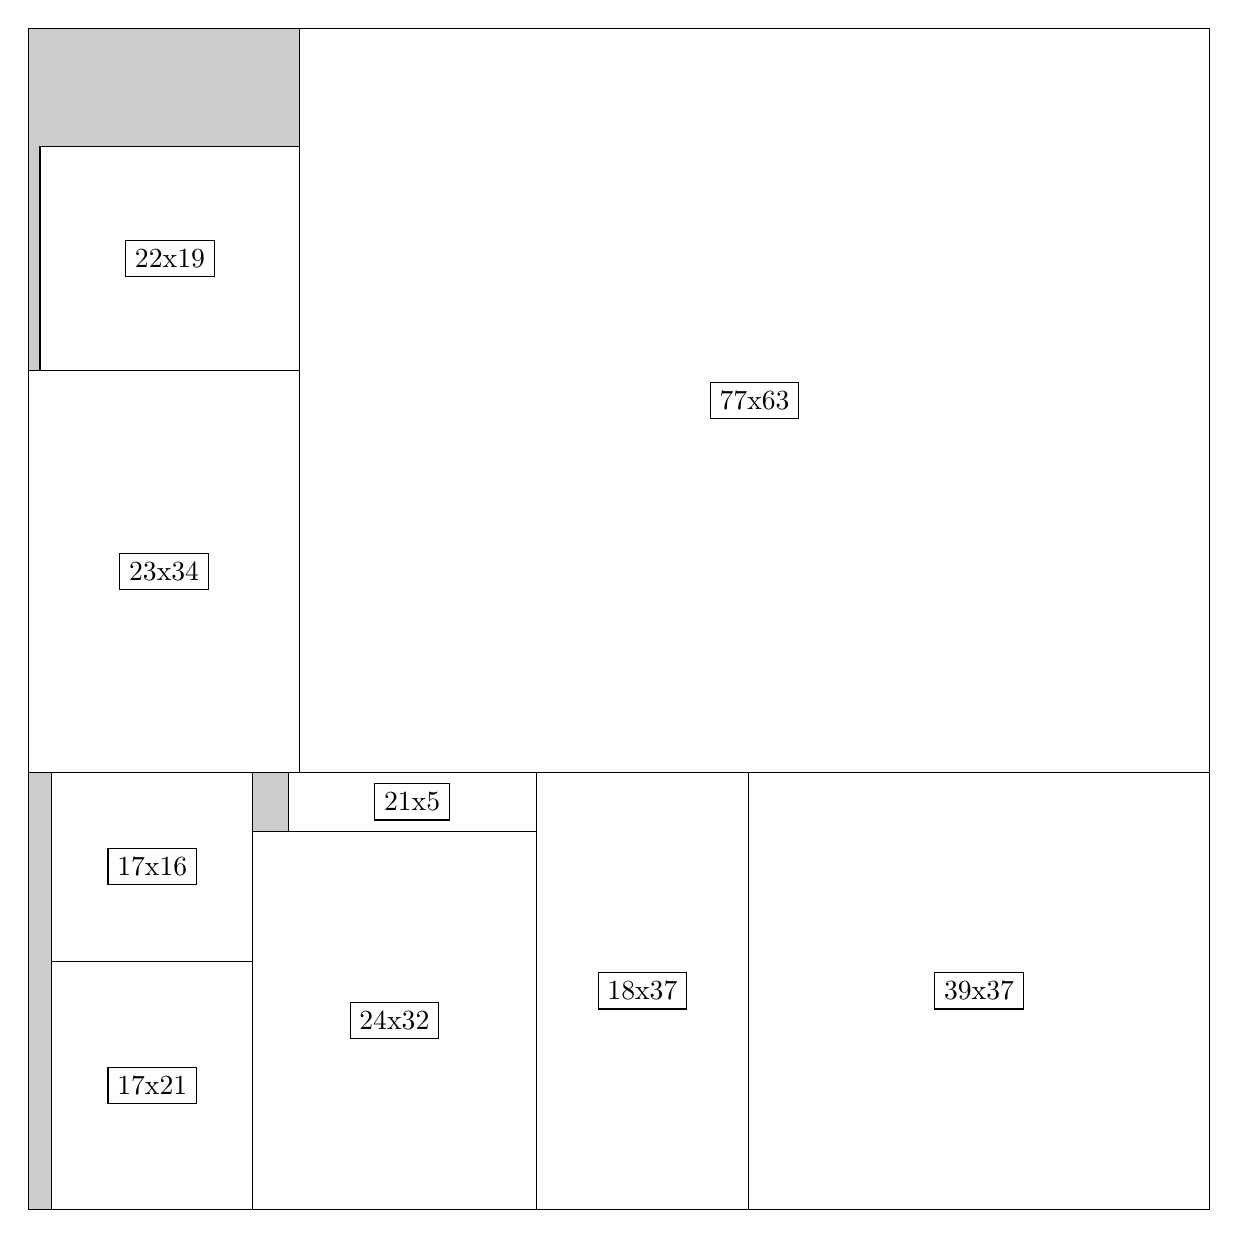
\begin{tikzpicture}[shorten >=1pt,scale=1.0,every node/.style={scale=1.0},->]
\tikzstyle{vertex}=[circle,fill=black!25,minimum size=14pt,inner sep=0pt]
\filldraw[fill=gray!40!white, draw=black] (0,0) rectangle (15.0,15.0);
\foreach \name/\x/\y/\w/\h in {39x37/9.15/0.0/5.85/5.55,18x37/6.45/0.0/2.6999999999999997/5.55,24x32/2.85/0.0/3.5999999999999996/4.8,21x5/3.3/4.8/3.15/0.75,17x21/0.3/0.0/2.55/3.15,17x16/0.3/3.15/2.55/2.4,77x63/3.4499999999999997/5.55/11.549999999999999/9.45,23x34/0.0/5.55/3.4499999999999997/5.1,22x19/0.15/10.65/3.3/2.85}
\filldraw[fill=white!40!white, draw=black] (\x,\y) rectangle node[draw] (\name) {\name} ++(\w,\h);
\end{tikzpicture}


w =39 , h =37 , x =61 , y =0 , v =1443
\par
w =18 , h =37 , x =43 , y =0 , v =666
\par
w =24 , h =32 , x =19 , y =0 , v =768
\par
w =21 , h =5 , x =22 , y =32 , v =105
\par
w =17 , h =21 , x =2 , y =0 , v =357
\par
w =17 , h =16 , x =2 , y =21 , v =272
\par
w =77 , h =63 , x =23 , y =37 , v =4851
\par
w =23 , h =34 , x =0 , y =37 , v =782
\par
w =22 , h =19 , x =1 , y =71 , v =418
\par
\newpage


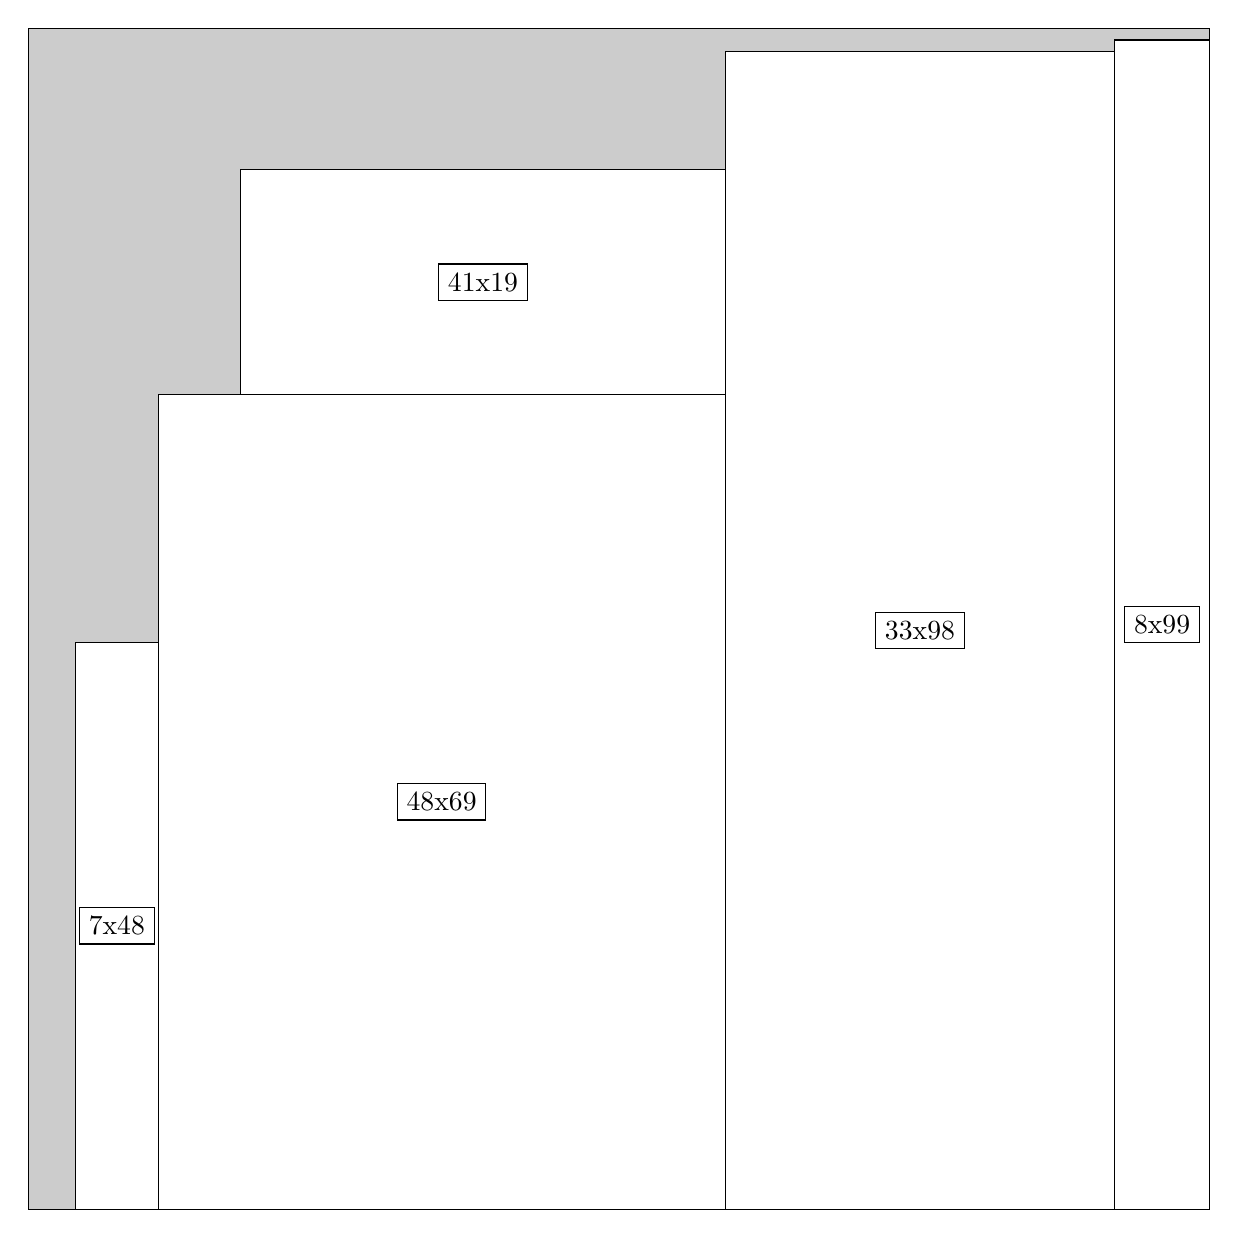
\begin{tikzpicture}[shorten >=1pt,scale=1.0,every node/.style={scale=1.0},->]
\tikzstyle{vertex}=[circle,fill=black!25,minimum size=14pt,inner sep=0pt]
\filldraw[fill=gray!40!white, draw=black] (0,0) rectangle (15.0,15.0);
\foreach \name/\x/\y/\w/\h in {8x99/13.799999999999999/0.0/1.2/14.85,33x98/8.85/0.0/4.95/14.7,48x69/1.65/0.0/7.199999999999999/10.35,41x19/2.6999999999999997/10.35/6.1499999999999995/2.85,7x48/0.6/0.0/1.05/7.199999999999999}
\filldraw[fill=white!40!white, draw=black] (\x,\y) rectangle node[draw] (\name) {\name} ++(\w,\h);
\end{tikzpicture}


w =8 , h =99 , x =92 , y =0 , v =792
\par
w =33 , h =98 , x =59 , y =0 , v =3234
\par
w =48 , h =69 , x =11 , y =0 , v =3312
\par
w =41 , h =19 , x =18 , y =69 , v =779
\par
w =7 , h =48 , x =4 , y =0 , v =336
\par
\newpage


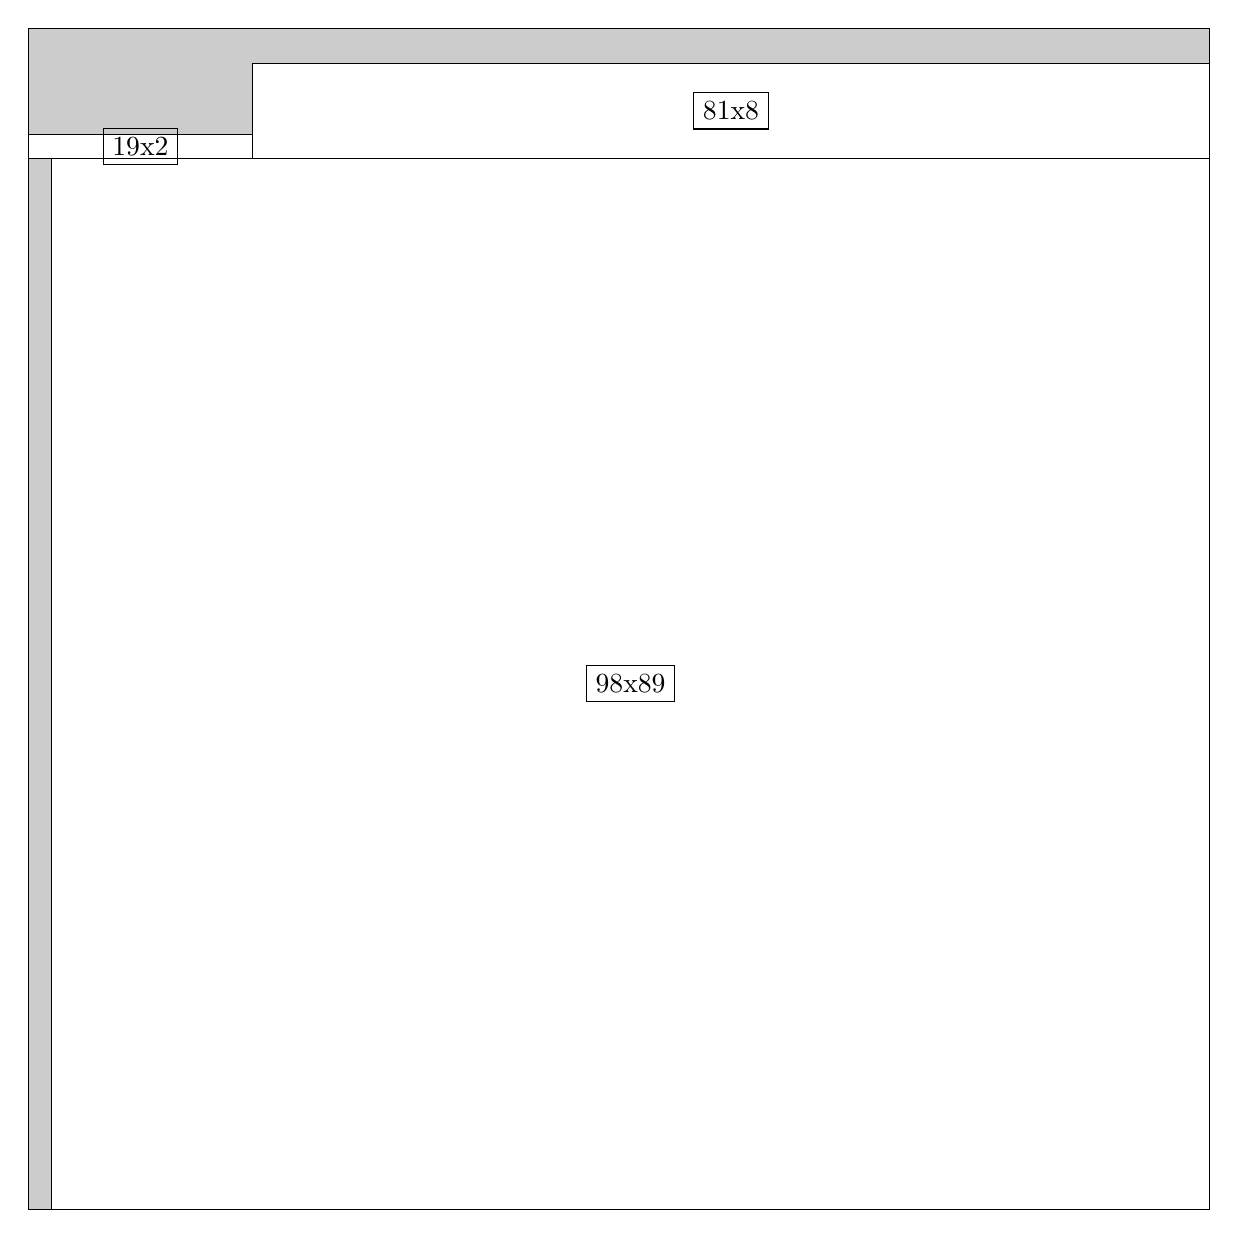
\begin{tikzpicture}[shorten >=1pt,scale=1.0,every node/.style={scale=1.0},->]
\tikzstyle{vertex}=[circle,fill=black!25,minimum size=14pt,inner sep=0pt]
\filldraw[fill=gray!40!white, draw=black] (0,0) rectangle (15.0,15.0);
\foreach \name/\x/\y/\w/\h in {98x89/0.3/0.0/14.7/13.35,81x8/2.85/13.35/12.15/1.2,19x2/0.0/13.35/2.85/0.3}
\filldraw[fill=white!40!white, draw=black] (\x,\y) rectangle node[draw] (\name) {\name} ++(\w,\h);
\end{tikzpicture}


w =98 , h =89 , x =2 , y =0 , v =8722
\par
w =81 , h =8 , x =19 , y =89 , v =648
\par
w =19 , h =2 , x =0 , y =89 , v =38
\par
\newpage


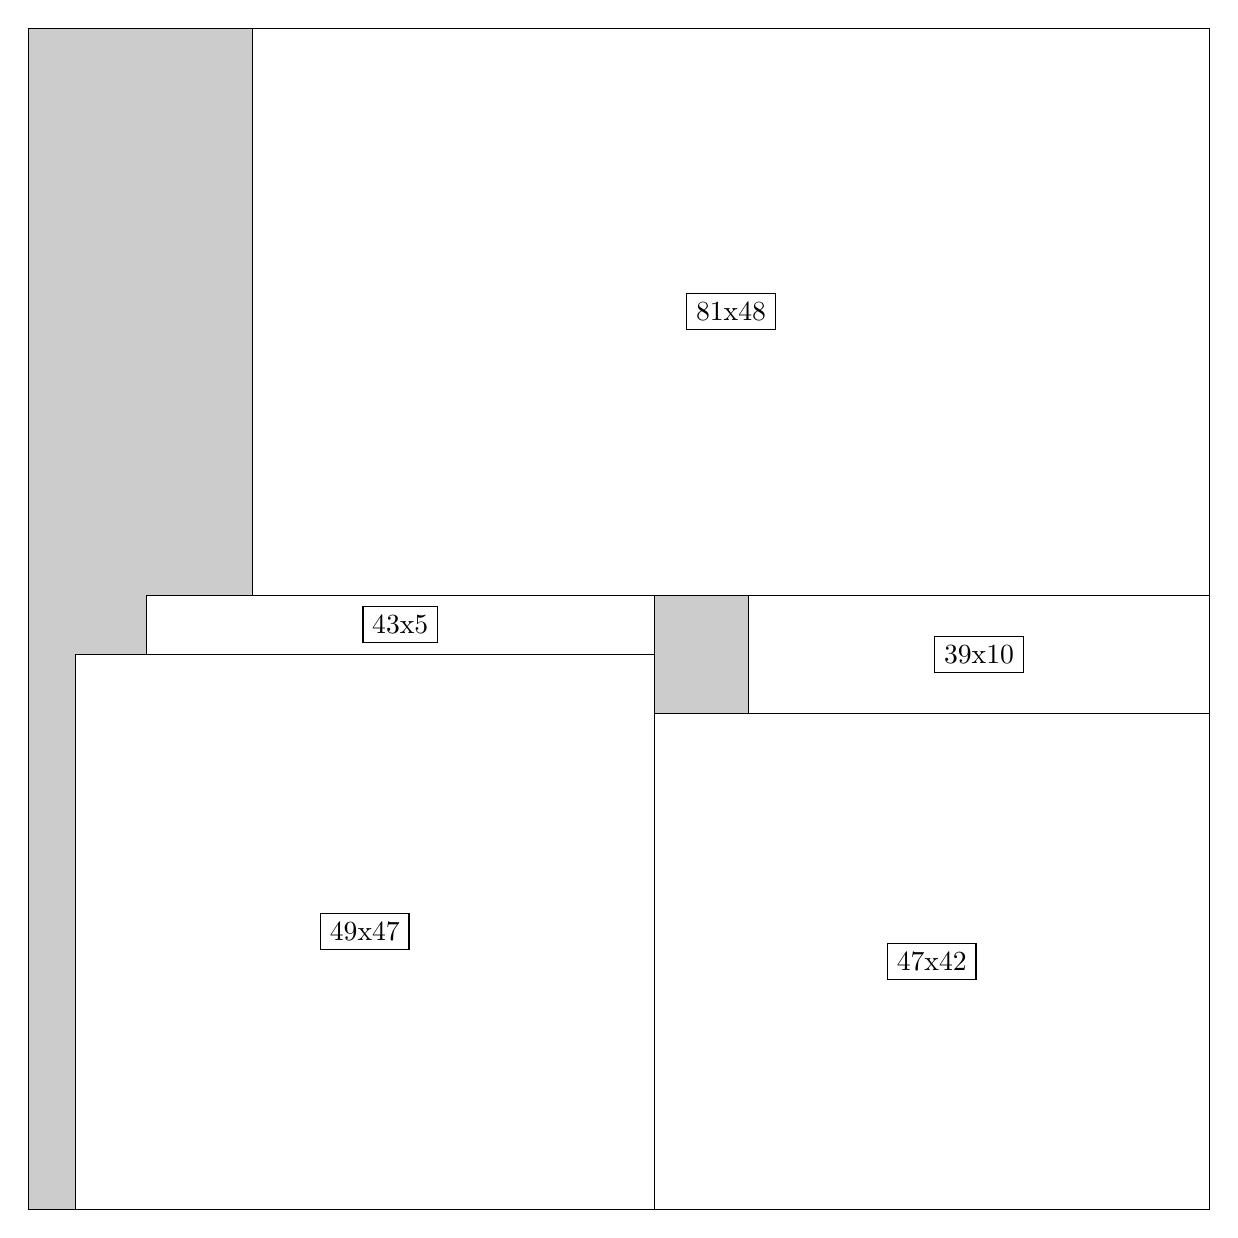
\begin{tikzpicture}[shorten >=1pt,scale=1.0,every node/.style={scale=1.0},->]
\tikzstyle{vertex}=[circle,fill=black!25,minimum size=14pt,inner sep=0pt]
\filldraw[fill=gray!40!white, draw=black] (0,0) rectangle (15.0,15.0);
\foreach \name/\x/\y/\w/\h in {47x42/7.949999999999999/0.0/7.05/6.3,39x10/9.15/6.3/5.85/1.5,49x47/0.6/0.0/7.35/7.05,43x5/1.5/7.05/6.45/0.75,81x48/2.85/7.8/12.15/7.199999999999999}
\filldraw[fill=white!40!white, draw=black] (\x,\y) rectangle node[draw] (\name) {\name} ++(\w,\h);
\end{tikzpicture}


w =47 , h =42 , x =53 , y =0 , v =1974
\par
w =39 , h =10 , x =61 , y =42 , v =390
\par
w =49 , h =47 , x =4 , y =0 , v =2303
\par
w =43 , h =5 , x =10 , y =47 , v =215
\par
w =81 , h =48 , x =19 , y =52 , v =3888
\par
\newpage


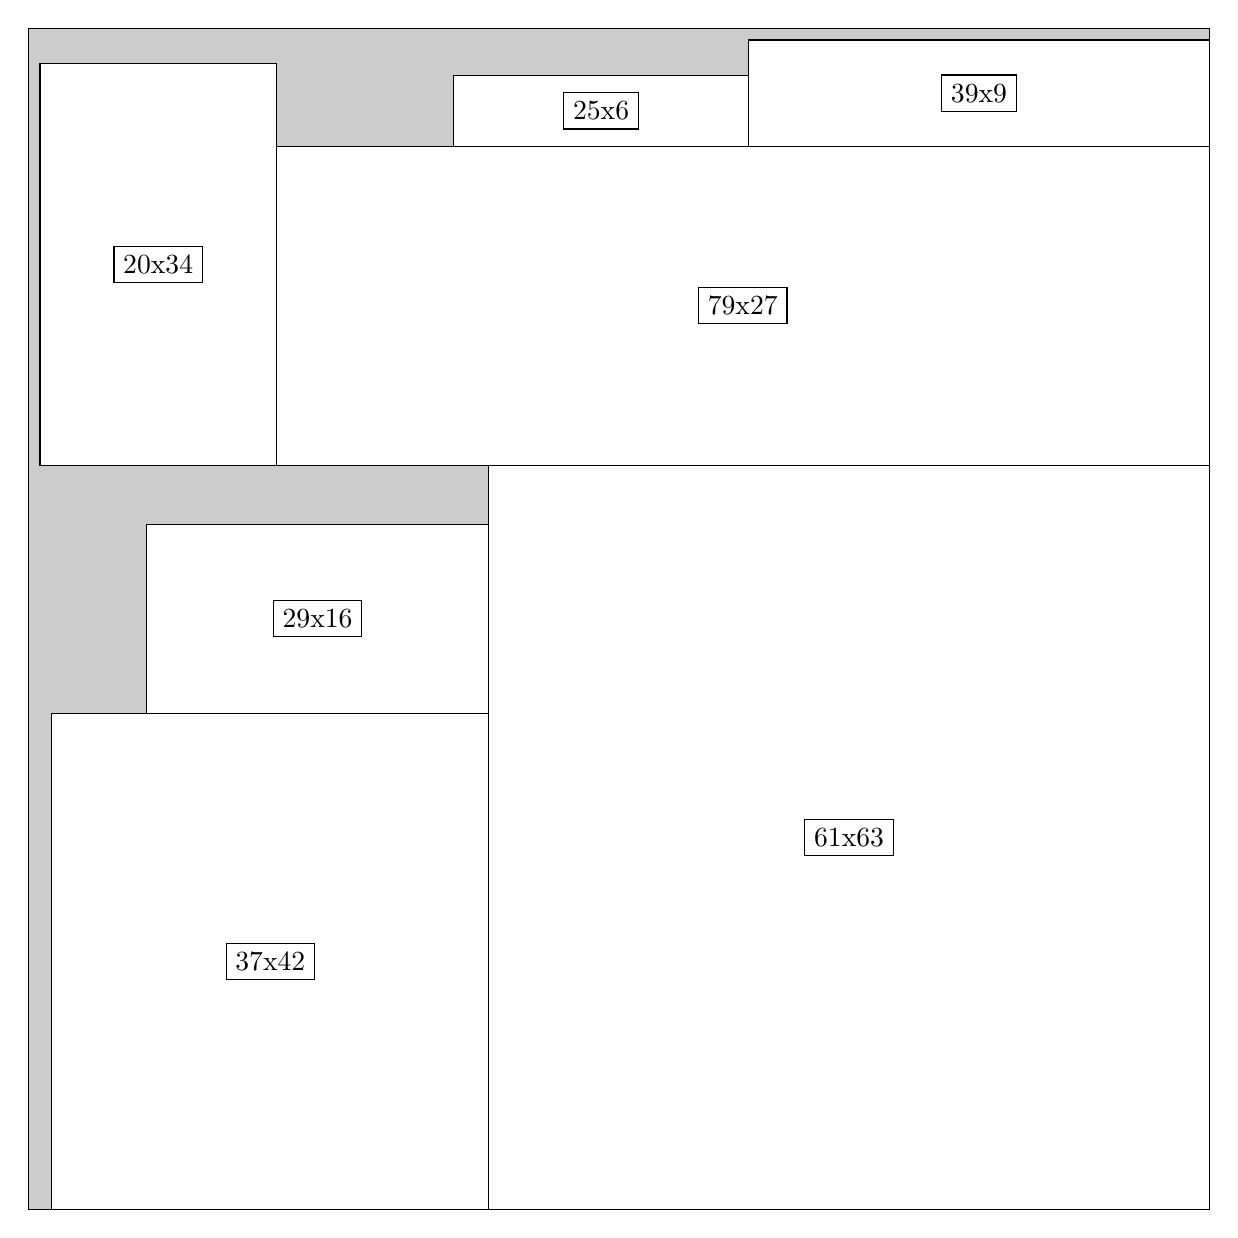
\begin{tikzpicture}[shorten >=1pt,scale=1.0,every node/.style={scale=1.0},->]
\tikzstyle{vertex}=[circle,fill=black!25,minimum size=14pt,inner sep=0pt]
\filldraw[fill=gray!40!white, draw=black] (0,0) rectangle (15.0,15.0);
\foreach \name/\x/\y/\w/\h in {61x63/5.85/0.0/9.15/9.45,37x42/0.3/0.0/5.55/6.3,29x16/1.5/6.3/4.35/2.4,79x27/3.15/9.45/11.85/4.05,39x9/9.15/13.5/5.85/1.3499999999999999,25x6/5.3999999999999995/13.5/3.75/0.8999999999999999,20x34/0.15/9.45/3.0/5.1}
\filldraw[fill=white!40!white, draw=black] (\x,\y) rectangle node[draw] (\name) {\name} ++(\w,\h);
\end{tikzpicture}


w =61 , h =63 , x =39 , y =0 , v =3843
\par
w =37 , h =42 , x =2 , y =0 , v =1554
\par
w =29 , h =16 , x =10 , y =42 , v =464
\par
w =79 , h =27 , x =21 , y =63 , v =2133
\par
w =39 , h =9 , x =61 , y =90 , v =351
\par
w =25 , h =6 , x =36 , y =90 , v =150
\par
w =20 , h =34 , x =1 , y =63 , v =680
\par
\newpage


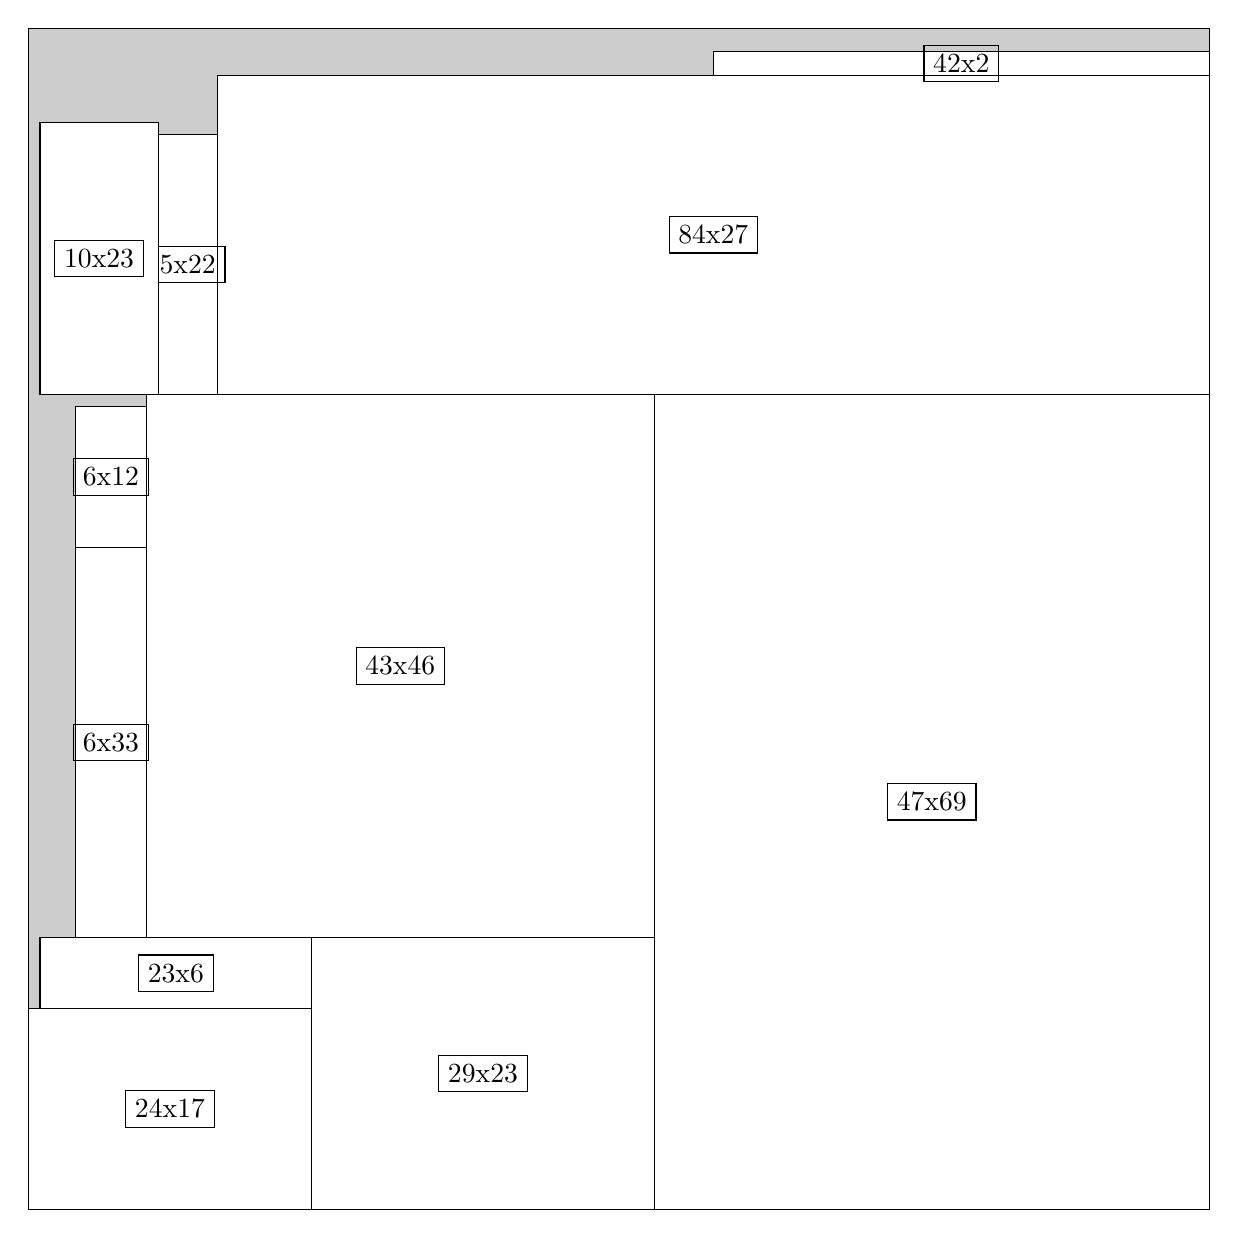
\begin{tikzpicture}[shorten >=1pt,scale=1.0,every node/.style={scale=1.0},->]
\tikzstyle{vertex}=[circle,fill=black!25,minimum size=14pt,inner sep=0pt]
\filldraw[fill=gray!40!white, draw=black] (0,0) rectangle (15.0,15.0);
\foreach \name/\x/\y/\w/\h in {47x69/7.949999999999999/0.0/7.05/10.35,29x23/3.5999999999999996/0.0/4.35/3.4499999999999997,24x17/0.0/0.0/3.5999999999999996/2.55,23x6/0.15/2.55/3.4499999999999997/0.8999999999999999,43x46/1.5/3.4499999999999997/6.45/6.8999999999999995,6x33/0.6/3.4499999999999997/0.8999999999999999/4.95,6x12/0.6/8.4/0.8999999999999999/1.7999999999999998,84x27/2.4/10.35/12.6/4.05,42x2/8.7/14.399999999999999/6.3/0.3,5x22/1.65/10.35/0.75/3.3,10x23/0.15/10.35/1.5/3.4499999999999997}
\filldraw[fill=white!40!white, draw=black] (\x,\y) rectangle node[draw] (\name) {\name} ++(\w,\h);
\end{tikzpicture}


w =47 , h =69 , x =53 , y =0 , v =3243
\par
w =29 , h =23 , x =24 , y =0 , v =667
\par
w =24 , h =17 , x =0 , y =0 , v =408
\par
w =23 , h =6 , x =1 , y =17 , v =138
\par
w =43 , h =46 , x =10 , y =23 , v =1978
\par
w =6 , h =33 , x =4 , y =23 , v =198
\par
w =6 , h =12 , x =4 , y =56 , v =72
\par
w =84 , h =27 , x =16 , y =69 , v =2268
\par
w =42 , h =2 , x =58 , y =96 , v =84
\par
w =5 , h =22 , x =11 , y =69 , v =110
\par
w =10 , h =23 , x =1 , y =69 , v =230
\par
\newpage


\end{document}